\documentclass[main.tex]{subfiles}
% CONCEPTS
\begin{document}
  % Data Structure
  % Trace by Trace Anaysis
    % Points of Interest
    % Polynomal
    % Exponential
  % Limitations
    % Trigonometric
      % Use FFT
    % Nested Functions
    % Noise vs Precision
      % Typical Trade Off
      
  \section{Numerical Derivative}
    
    Taking the derivative in a discrete Data Set.
    \[Matrix\]
    Explain \textit{derivDepth} and the tails that show \textit{POI}.
    \\\\
    Try to accompany Tables with Graphs of the function.
  
  \section{Derivative Characteristics}
    
    By far the simplest functions to classify are \textbf{polynomials}. Any polynomial of degree $N$ will have exactly $N$ non-zero derivatives, and so it is only necessary to count the number of times that the derivative is not zero. If it never becomes zero then the data is not polynomial, or we have not taken enough derivatives.
          
    \begin{figure}[h]
      \begin{subfigure}{0.48\linewidth}
        \centering
        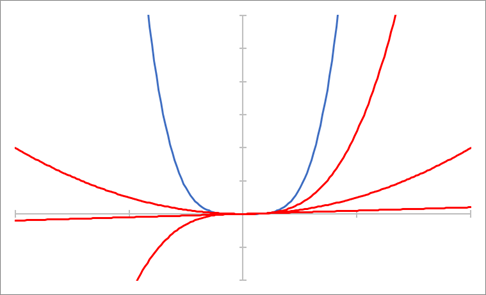
\includegraphics[width=0.9\linewidth]{figures/derivPoly}
        \caption{Polynomials}
        \label{fig:deriv:poly}
      \end{subfigure}
      \begin{subfigure}{0.48\linewidth}
        \centering
        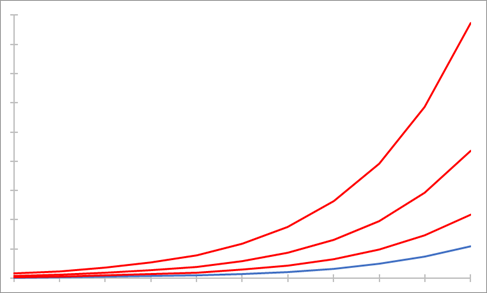
\includegraphics[width=0.9\linewidth]{figures/derivExp}
        \caption{Exponential}
        \label{fig:deriv:exp}
      \end{subfigure}
      \caption{Derivative patterns of (\subref{fig:deriv:poly}) polynomial and \subref{fig:deriv:exp}) exponential functions. (\subref{fig:deriv:poly}) shows a fourth order polynomial in blue ($x^4$) and its derivatives in red, a third ($x^3$), second ($x^2$) and first ($x$) order polynomial, which a "zeroth" order polynomial ($x^0$ or simply $1$) follows, but is too small do display. No further derivatives would follow. (\subref{fig:deriv:exp}) shows an exponential of the form $e^{a x}$ in blue, with $a>1$ and hence its derivatives growing larger with the level of derivative, by $a$, $a^2$ and $a^3$ respectively. (\subref{fig:deriv:exp}) will never reach a zero derivative.}
      \label{fig:deriv}
    \end{figure}
  
  \section{Trace by Trace Analysis}
  \subsection{Principle}
  Make use of Tables here
  
  \subsection{Detectable Phenomena}
  
  \subsubsection{Data Points of Interest}
  When the derivatives change (from linear to square etc. Use tables to show what happens) This is used to mark "data points of interest" i.e. changes of function, bias or obvious outliers (based on precision used).
  
  \[Tables-of-changes\]
  
  A Bias is when all data points after this point are higher or lower independent of the derivative. This is relatively common in sensor readings e.g. when an interferometer is *knocked* and subsequent measurements are off by a set amount. It is a common form of systematic error, but can easily be corrected for by adding or subtracting the difference from the subsequent data points to *reallign* them.
  
  \[Image of Bias Data\]
  
  Outliers,  strongly affected by the desired precision
  
  Downside of this method is that all data points before those of interest are affected by the derivatives. This is affected by the depth of the calculated derivatives and can hide other interesting data points. However, as the depth of derivative are not usually above $10$ and all intended applications involve data points of the order of $10^3$ or more, this is considered a minor flaw.
  
  \subsubsection{Polynomial Data}
  
  The simplest Data that can be classified in this way is polynomial data i.e. data conforming to the form $y= \sum_{i=0}^{D} a_i x^i$ (where $D$ is the degree of the polynomial and \( i \in \mathbb{Z}^\geq \) ), for example in parabolas like $y=a x^2 + b x +c$ or linear functions as $y=a x + b$. This data is representative of many pphysical phenomena, from the air resistance to the charging of a capacitor [cite Tippler].
  
  \[Plots-of-some-of-these-formulas-or-phenomena\]
  
  This Data is easily detected by  the system as it has only a limited number of derivatves that are not zero. Since the derivative of a polynomial of degree $D$ is of the degree $D-1$, continuing to calculate the derivative, whether analytically or numerically, will produce exactly $D$ non-zero derivatives. Provided that the depth to which derivatives are calculated is larger than $D$ these can be counted easily.
  
  \subsubsection{Simple Non-Polynomial Data}
  
  Non-Polynomial data differes significantly as it typically produces infinitlely non-zero derivatives. These include, most significantly, *exponential data* of the form $a e^{b x + c} + d$ (where $e$ is *Euler's Constant*), trigonometric data as in $a \sin(\theta +b) + c$, among others. 
  
  Perhaps the most common function modelling physical phenomena is the *exponential*, representing phenomena like *population growth* or *nuclear decay* accurately.  In its simplest form $y=e^x$ it is well known for being its own derivative, which continues infinitely. However, it can easily be converted to a linear function of the form $y=a x+b$ by taking the natural logarithm of all data points. This is commonly done to allow regression over exponential data [citation needed], and allows the application to accurately classify exponential data. Whenever sections of data have infinite derivatives the logarithm is taken, if the second derivative is zero it is exponential.
  
  Trigonometric Data  can be classified in much the same way, by taking the $\arcsin(\theta)$ of the data points and checking, as before, if the second derivative is zero. Because $\sin(\frac{\pi}{2}-\theta)=\cos(\theta)$ and data is assumed to be of the form $a \sin( \theta + b)+c$ this is sufficient to classify this data.
  
  \subsubsection{Unclassifiable Functions}
  
  Some phenomena can be described by functions of polynomial form, but by allowing non-integer or negative values, like this: $y=\sum_i a_i x^i$ where $i \in \mathbb{Q} $.   The simplest and most comm example of this is $y=\frac{1}{g_{(x)}}=g_{(x)}^{-1}$, which is involved in many functions, like that for *gravitational force* $F_g=\frac{G m_1 m_2}{r^2}$ [cite tippler equ. 11-5 p. 367]. This particular function can be easily classified by taking the reciprocal and then classifying as normal.
  
  In principle, these phenomena are normally functions of nested functions to form $f(g_{(x)})$. Some examples include the *driven RLC Circuit* of the form $P_{av}= \frac{ (V_{app\_rms})^2R\omega^2 }{ L^2(\omega^2-\omega_0^2)^2+\omega^2R^2 }$  [cite tippler equ. 29-56, p. 1014.] or, famously, relativistic momentum $p=\frac{m v}{\sqrt{1-(v^2/c^2)}}$ [cite tippler equ R-10] or indeed the *gravitational force* example from above. The former example nests functions of the form $f(g_{(x)},h_{(y)})=g_{(x)}h_{(x)}^{-1}$ with several second order polynomials, while Einstein's further involves $y=g_{(x)}^{\frac{1}{2}}$.
  
  In order to classify these more complex nestings the application would be forced to unwrap each step of nesting with the correct reverse function, which in turn must be found largely by trial and error. This combinatorial explosion of possibilities means that, especially for larger data sets, at this time, no good way of classifying nested functions is available and human analysis is still required.
  
  \subsubsection{Nested Analysis}
  
  As discussed above, DataSet Instances can be nested to model higher dimensions. Provided the nested instances are standardiseed as in the `NestedValueDataSet` data can be accessed and analysed across rather than along the ValueDataSet instances [fig.]. 
  
  \[Illustrate-NestedValueDataSet-with-ValueDataSet-inside-for-3D-data\]
  
  This may be slightly less advantagous compared to along the set analysis in terms of computing resources, it does allow properly modelling higher dimensional data. 
  
  Maybe talk about computational penalties? 
  
  \subsection{Limitations}
  \subsubsection{Noise and Precision}
  Precision is key here. Noise can be ignored by reducing precision, while outliers can e detected by increasing it. There is an obvious balance to be struck.
  
  Luckily precision in analysis does not affect processing cost.
  \subsubsection{Processing}
  Adjusting precision is free.
  
  In higher dimensional analysis it should be kept in mind that analysis along the set is cheaper than across. Hence there is always one dimension along which analysis is cheapest, which should be the dimension with the highest potential.
  
  For the intended applications caching will have to be introduced as data sets are large. This is an unavoidable limitation, [calculate some examples or find a more general approach to find  the costs relative to data set size]
  \subsubsection{Similar Functions?}
  
  
\end{document}